%!TEX root = ../dokumentation.tex

\chapter{Analyse}
Bei der Software-Entwicklung werden unterschiedliche Entwicklungsschritte
durchlaufen. Dieser Entwicklungsverlauf wird allgemein auch als \ac{SDLC} bezeichnet
und unterscheidet die folgenden Phasen:
\begin{figure}[h]
    \centering
    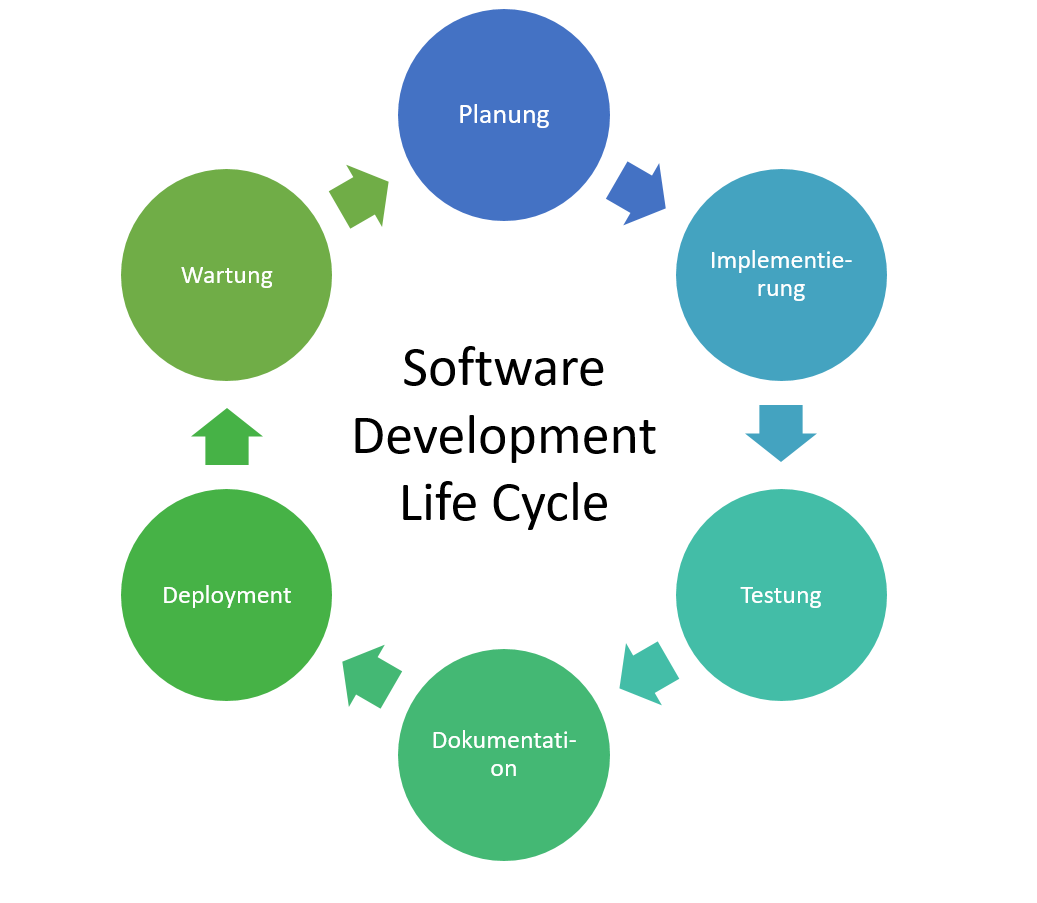
\includegraphics[scale=0.3]{SDLC.png}
    \caption{\acl{SDLC}}
\end{figure}

\begin{comment}
\item Planung
\item Implementierung
\item Testung
\item Dokumentation
\item Deployment
\item Wartung
\end{comment}

Die Phase der Planung ist eine der wichtigsten Phase im ganzen
Entwicklungsprozess. Hier werden die Anforderungen an das Projekt definiert 
und erste Analysen zur Umsetzung vollzogen \autocite{SDLC_2019}. Die
Anforderungsanalyse wurde bereits im ersten Kapitel der Arbeit in Form des Ist-
und Soll-Zustandes erörtert und die damit vorliegende Problemstellung
offengelegt. \newline 
In diesem Kapitel soll nun auf die verschiedenen
Möglichkeiten bei der Umsetzung eingegangen werden. Darunter fällt vor allem
der Vergleich verschiedener Technologien und Bibliotheken, welche später bei
der Implementierung eingesetzt werden könnten. 


\section{Einarbeitung}
Bevor es an die Realisierung der Aufgabe geht, steht zunächst das
Vertrautmachen mit den unterschiedlichen Technologien im Vordergrund. Für die
Entwicklung wurde eine Raspberry Pi 3 Modell B bereitgestellt. Da das zu
entwickelnde Programm später auf dem gleichen Modell laufen soll, wird auf
einen Vergleich der verschiedenen Modelle verzichtet. Bevor der Raspberry Pi
benutzt werden kann, muss zunächst ein Betriebssystem installiert werden.
\hfill \break

Für den Raspberry Pi gibt es verschiedene Distributionen, die auf verschiedene
Anwendungsszenarien ausgelegt sind. Nachfolgend ist ein Auszug aus den verfügbaren
Betriebssystem aufgelistet: 
\begin{description}
\item[Raspbian] \hfill \\ 
    Raspbian ist eines der ältesten und meist verbreitetsten Betriebssysteme für
    den Raspberry Pi. 
\item[Pi MusicBox] \hfill \\ 
    Bei der Pi MusicBox handelt es sich um eine Distribution, welche auf das
    Abspielen von Musik ausgelegt ist. Es unterstützt alle bewährten
    Streaming-Dienste oder auch das Streamen von Musik aus dem Netzwerk.
\item[RetroPie] \hfill \\
    Der RetroPie ist eine Distribution, welche das Emulieren von klassischen
    Spielkonsolen ermöglicht.
\end{description}

Im Rahmen dieser Arbeit geht es zwar um das Abspielen von Audiodateien,
allerdings soll dafür ein eigenständiges Tool entwickelt werden. Da Raspbian
das offizielle Betriebssystem für den Raspberry Pi ist, es dafür die meisten
Pakete gibt und es am weitesten verbreitet ist, wird sich im Bezug auf diese
Arbeit für das Betriebssystem Raspbian entschieden
\autocite{Best_Raspberry_Pi_distros_2019}.
\hfill \break

Um Raspbian auf dem Raspberry Pi zu installieren gibt es zwei Möglichkeiten:
\ac{NOOBS} oder Raspbian. \ac{NOOBS} ist ein \ac{OSI}, welche durch seine Einfachheit besonders anfängerfreundlich ist.
Standardmäßig kommt er mit einer Installation von Raspbian und LibeELEC, kann
aber zusätzlich noch weitere Betriebssysteme laden. Wenn man nur Raspbian
verwenden will, kann man sich die Installation von \ac{NOOBS} sparen und direkt
Raspbian nutzen. Da wir in unserem Projekt auch nur Raspbian verwenden werden,
haben wir uns für die zweite Variante entschieden \autocite{monk_2019}.


\section{Abspielen von Audiodateien}
Im ersten Schritt der Analyse geht es an die Entscheidung einer geeigneter
Audiobibliothek, um das Abspielen von Audiodateien zu ermöglichen. Wichtig
dabei ist, dass die Bibliothek keine Einschränkungen bei der Benutzung hat, gut
dokumentiert ist und bestenfalls eine bestehende Schnittstelle für Go besitzt.

\subsection{Bibliotheken}
\paragraph{PortAudio}
PortAudio ist eine Open Source Bibliothek, welche das Abspielen und Aufnehmen
von Audiodateien ermöglicht. Sie bietet eine plattformübergreifende Lösung,
wodurch sie auf den gängigsten Betriebssystemen problemlos läuft. Einer der
Gründe dafür, dass sie plattformübergreifend funktioniert, ist der, dass
PortAudio in der Programmiersprache C geschrieben wurde. \hfill

Die Kommunikation mit PortAudio verläuft über eine \ac{API} Schnittstelle.
Diese nimmt den Datenstrom entgegen, welcher abgespielt werden soll. Während
des Abspiel- oder Aufnahmeprozesses von Audiodateien benutzt PortAudio entweder
eine Callback-Funktion oder ein blockierendes Read/Write Interface
\autocite{PortAudio_2019}.

\paragraph{libsoundio}
libsoundio ist genau wie PortAudio eine Open Source Bibliothek, die eine
Schnittstelle zur Ein- und Ausgabe von Audiostreams bietet. Sie zeichnet
sich durch ihre Plattformunabhängigkeit und ihre sehr gute Dokumentation aus.
libsoundio stellt eine leichtgewichtige Abstraktion über verschiedenste
Soundtreiber dar \autocite{libsoundio_2019}.

\subsection{Entscheidung}
Nach einigen Recherchen konnten keine großartigen Unterschiede zwischen den
beiden Grundkonzepten der Audiobibliotheken festgestellt werden. Ein Vorteil von
libsoundio ist ganz klar, dass sie eine ausgesprochen umfangreiche
Dokumentation besitzt, in der der Entwickler einen großen Fokus auf
Vollständigkeit gelegt hat. PortAudio hingegen ist im Gegenzug weiter verbreitet.
Da Go eine Bibliothek bietet, welche im Hintergrund auf die Schnittstelle
von PortAudio zurückgreift, wird sich im Rahmen der Arbeit für die
Verwendung von PortAudio entschieden.

\section{MP3 Decoder}
Bei \ac{MP3}-Dateien handelt es sich um komprimierte Audio-Dateien. Im
Vergleich zu anderen Audioformaten, setzt \ac{MP3} auf das
Psychoakustik-Modell. Dieses besagt, dass Menschen nur in einer Frequenz von 20
Hz bis 20 kHz hören kann. \ac{MP3} filtert deshalb alle anderen für den
Menschen nicht hörbaren Bereich raus, und erreicht so eine Speicherersparnis um
mehr als den Faktor 10 im Vergleich zum Rohformat. Auch durch die geringe
Speichergröße hat sich \ac{MP3} zu einer der weitverbreitetsten Formate für
Audiodateien entwickelt.  Deshalb sollte dieses Format unbedingt auch durch den
zu entwickelnden Audioplayer unterstützt werden \autocite{mp3}. \hfill

Um die Unterstützung für das Abspielen von \ac{MP3}-Dateien zu ermöglichen,
muss bei der Implementierung auf einen \ac{MP3} Decoder zur Dekodierung
der \ac{MP3}-Dateien zurückgegriffen werden. Für diesen Zweck wird sich für die
Go-Bibliothek \textit{go-mpg123}. Diese greift im
Hintergrund auf die Bibliothek \textit{libmpg123} zu. Aktuell befindet sich die
Bibliothek noch in der Entwicklung, jedoch bietet sie bereits die
geforderte Funktionalität zur Dekodierung an \autocite{mp3_decoder}.

\section{MP3 Tag Info Reader}
\ac{MP3} Dateien können neben den reinen Audiodaten auch noch zusätzliche
Informationen (Metadaten) speichern. Dafür verwendet \ac{MP3} ein Format namens
\ac{ID3}, welches einzelne Information in
sogenannten \textit{\ac{ID3}-Tags} speichert. In diesen Tags werden meist
Informationen wie Interpreten, Titel oder auch Albumname gespeichert. Da diese
Informationen in einem Audioplayer optimalerweise angezeigt werden sollten,
muss nach einer Möglichkeit zum Auslesen dieser Tags gesucht werden \autocite{id3}. \hfill
\break
Aktuell unterstützt \textit{go-mpg123} noch nicht das Auslesen der \ac{ID3}-Tags.
Deswegen muss nach einer anderen Bibliothek zur Auslesung dieser Daten gesucht
werden. Die Entscheidung fiel dabei auf die Go-Bibliothek \textit{ID3 Decoder},
da diese einfach zu verwenden ist und die meistverbreitetste Go-Bibliothek
für diesen Zweck ist \autocite{id3_go_2015}.
